\documentclass{report}
\usepackage[showframe=false]{geometry}
\usepackage{titlesec}
\usepackage{amsmath}
\usepackage{graphicx}
\usepackage{float}

\pagenumbering{gobble}

\geometry{tmargin=60pt,bmargin=90pt,lmargin=90pt,
rmargin=90pt}

\titleformat{\chapter}{\normalfont\huge}{\thechapter.}{20pt}{\huge}
\titlespacing*{\chapter} {0pt}{0pt}{10pt}

\begin{document}

\chapter{Section 1}

\begin{subequations}
  Starting Equations:
  \begin{flalign*}
    class1: A = [2, 2]^T, B = [3, 5]^T \\
    class1\_bias: A = [1, 2, 2]^T, B = [1, 3, 5]^T \\
    class2: C = [1, 3]^T, D = [-1, -0.5]^T \\
    class2\_bias: C = [1, 1, 3]^T, D = [1, -1, -0.5]^T \\
    initial\_weight\_vector: W0 = [1, 1, 1]^T
  \end{flalign*}
\end{subequations}


\begin{subequations}
  First Step of weight vector updating:
  \begin{flalign*}
    W0 * A = 5 (OK) \\
    W0 * B = 9 (OK) \\
    W0 * C = 5 (NOT OK) \\
    W1 = W0 - C = [0, 0, -2] \\
    W1 * D = 1 (NOT OK) \\
    W2 = W1 - D = [-1, 1, -1.5]
  \end{flalign*}
\end{subequations}

\begin{subequations}
  Second Step of weight vector updating:
  \begin{flalign*}
    W2 * A = -2 (NOT OK) \\
    W3 = W2 + A = [0, 3, 0.5] \\
    W3 * B = 11.5 (OK) \\
    W3 * C = 4.5 (NOT OK) \\
    W4 = W3 - C = [-1, 2, -2.5] \\
    W4 * D = -1.75 (OK) \\
  \end{flalign*}
\end{subequations}

\begin{subequations}
  Third Step of weight vector updating:
  \begin{flalign*}
    W4 * A = -2 (NOT OK) \\
    W5 = W4 + A = [0, 4, -0.5] \\
    W5 * B = 9.5 (OK) \\
    W5 * C = 2.5 (NOT OK) \\
    W6 = W5 - C = [-1, 3, -3.5] \\
    W6 * D = -2.25 (OK) \\
  \end{flalign*}
\end{subequations}

\begin{subequations}
  Four Step of weight vector updating:
  \begin{flalign*}
    W6 * A = -2 (NOT OK) \\
    W7 = W6 + A = [0, 5, -1.5] \\
    W7 * B = 7.5 (OK) \\
    W7 * C = 0.5 (NOT OK) \\
    W8 = W7 - C = [-1, 4, -4.5] \\
    W8 * D = -2.75 (OK)
  \end{flalign*}
\end{subequations}

\begin{subequations}
  Five Step of weight vector updating:
  \begin{flalign*}
    W8 * A = -2 (NOT OK) \\
    W9 = W8 + A = [0, 6, -2.5] \\
    W9 * B = 5.5 (OK) \\
    W9 * C = -1.5 (OK) \\
    W9 * D = -4.75 (OK) \\
  \end{flalign*}
\end{subequations}

\begin{subequations}
  Final result:
  \begin{flalign*}
    W9 * A = 7.000000 \\
    W9 * B = 5.500000 \\
    W9 * C = -1.500000 \\
    W9 * D = -4.750000 \\
    W9 = [0, 6, -2.5]
  \end{flalign*}
\end{subequations}


\chapter{Section 2}

\begin{verbatim}
By Hand:

  probability <- .6
  number_of_weak_learners <- 7
  x <- ceiling(number_of_weak_learners/2)
  final_sum <- 0

  for(i in number_of_weak_learners:x) {
    binomial_coefficient <- (factorial(number_of_weak_learners) / 
                                    (factorial(i) * factorial(number_of_weak_learners-i)))
    p <- probability^i
    np <- (1-probability)^(number_of_weak_learners-i)
    final_sum <- final_sum + (binomial_coefficient * p * np)
  }
  print(final_sum)

R Packages:
  final_sum <- dbinom(7, size=7, prob=0.6) + 
               dbinom(6, size=7, prob=0.6) + 
               dbinom(5, size=7, prob=0.6) + 
               dbinom(4, size=7, prob=0.6)
\end{verbatim}


ANSWER: 71.0208\% majority vote accuracy

\chapter{Section 3}

\begin{verbatim}
A <- c(2, 10)
B <- c(2, 5)
C <- c(8, 4)
D <- c(5, 8)
E <- c(7, 5)
F <- c(6, 4)
G <- c(1, 2)
H <- c(4, 9)
M <- c(3, 3)

class_1 <- rbind(A, B, G, H)
class_2 <- rbind(C, D, E, F)

M1 <- as.matrix(colMeans(class_1))

S1 <- (A-M1) %*% t(A - M1) +
      (B-M1) %*% t(B - M1) +
      (G-M1) %*% t(G - M1) +
      (H-M1) %*% t(H - M1)

M2 <- as.matrix(colMeans(class_2))

S2 <- (C-M2) %*% t(C - M2) +
      (D-M2) %*% t(D - M2) +
      (E-M2) %*% t(E - M2) +
      (F-M2) %*% t(F - M2)

S <- S1 + S2

W <- solve(S)%*%(M1-M2)

print(t(W)%*%M)

\end{verbatim}


\[
  class\_1 <- 
  \begin{bmatrix}
    2 & 10 \\
    2 & 5 \\
    1 & 2 \\
    4 & 9
  \end{bmatrix}
\]

\[
  class\_2 <- 
  \begin{bmatrix}
    8 & 4 \\
    5 & 8 \\
    7 & 5 \\
    6 & 4
  \end{bmatrix}
\]

\[
  M1 <- 
  \begin{bmatrix}
    2.25 \\
    6.50
  \end{bmatrix}
\]

\[
  M2 <- 
  \begin{bmatrix}
    6.50 \\
    5.25
  \end{bmatrix}
\]

\[
  S1 <- 
  \begin{bmatrix}
    4.75 & 9.50 \\
    9.50 & 41.0
  \end{bmatrix}
\]

\[
  S2 <- 
  \begin{bmatrix}
    5.00 & -5.50 \\
    -5.50 & 10.75
  \end{bmatrix}
\]

\[
  S <- 
  \begin{bmatrix}
    9.75 & 4.00 \\
    4.00 & 51.75
  \end{bmatrix}
\]

\[
  W <- 
  \begin{bmatrix}
    -0.46040681 \\
    0.05974159
  \end{bmatrix}
\]

\[
  class\_1\_solution <- 
  \begin{bmatrix}
    -0.3233977 \\
    -0.6221057 \\
    -0.3409236 \\
    -1.303953
  \end{bmatrix}
\]

\[
  class\_2\_solution <- 
  \begin{bmatrix}
    -3.444288 \\
    -1.824101 \\
    -2.92414 \\
    -2.523474
  \end{bmatrix}
\]

\[
  unknown\_solution <- 
  \begin{bmatrix}
    -1.201996
  \end{bmatrix}
\]

Unknown Solution is in class 1
  

\chapter{Section 4}

\begin{verbatim}

entropy <- function(values) {
  total <- 0
  entropy_total <- 0
  for(i in 1:length(values)) { 
    total <- total + values[i]
  }

  for(i in 1:length(values)) { 
    entropy_total <- entropy_total + ((-values[i]/total) * log2(values[i]/total))
  }
  if(is.nan(entropy_total)) {
    return(0)
  }
  return(entropy_total)
}

info <- function(...) {
  input_list <- list(...)
  total <- 0
  for(i in 1:length(input_list)) {
    input <- input_list[[i]]
    for(x in 1:length(input)) {
      total <- total + input[x]
    }
  }

  Gain <- 0
  for(i in 1:length(input_list)) {
    input <- input_list[[i]]
    local_total <- 0
    for(x in 1:length(input)) {
      local_total <- local_total + input[x]
    }
    Gain <- Gain + ((local_total/total) * entropy(input))
  }
  return(Gain)
}

Color <- c("Red", "Blue", "Red", "Green", "Red", "Green")
Shape <- c("Square", "Square", "Round", "Square", "Round", "Square")
Size <- c("Big", "Big", "Small", "Small", "Big", "Big")
Class <- c("+", "+", "-", "-", "+", "-")

data <- data.frame(Color=Color, Shape=Shape, Size=Size, Class=Class)

negitive_count <- nrow(data[data$Class == "-",])
positive_count <- nrow(data[data$Class == "+",])

# Color = Red
color <- data[data$Color == "Red",]
color_red_negitive_count <- nrow(color[color$Class == "-",])
color_red_positive_count <- nrow(color[color$Class == "+",])

# Color = Blue
color <- data[data$Color == "Blue",]
color_blue_negitive_count <- nrow(color[color$Class == "-",])
color_blue_positive_count <- nrow(color[color$Class == "+",])

# Color = Green
color <- data[data$Color == "Green",]
color_green_negitive_count <- nrow(color[color$Class == "-",])
color_green_positive_count <- nrow(color[color$Class == "+",])

expected_color <- info(c(color_red_negitive_count, color_red_positive_count),
                       c(color_blue_negitive_count, color_blue_positive_count),
                       c(color_green_negitive_count, color_green_positive_count))

# Shape = Square
shape <- data[data$Shape == "Square",]
shape_square_negitive_count <- nrow(shape[shape$Class == "-",])
shape_square_positive_count <- nrow(shape[shape$Class == "+",])

# Shape = Round
shape <- data[data$Shape == "Round",]
shape_round_negitive_count <- nrow(shape[shape$Class == "-",])
shape_round_positive_count <- nrow(shape[shape$Class == "+",])

expected_shape <- info(c(shape_square_negitive_count, shape_square_positive_count),
                       c(shape_round_negitive_count, shape_round_positive_count))

# Size = Big
size <- data[data$Size == "Big",]
size_big_negitive_count <- nrow(size[size$Class == "-",])
size_big_positive_count <- nrow(size[size$Class == "+",])

# Size = Small
size <- data[data$Size == "Small",]
size_small_negitive_count <- nrow(size[size$Class == "-",])
size_small_positive_count <- nrow(size[size$Class == "+",])

expected_size <- info(c(size_big_negitive_count, size_big_positive_count),
                       c(size_small_negitive_count, size_small_positive_count))

gain_color <- info(c(positive_count, negitive_count)) - expected_color
gain_shape <- info(c(positive_count, negitive_count)) - expected_shape
gain_size <- info(c(positive_count, negitive_count)) - expected_size

print(sprintf("gain(Color)         = %s bits", gain_color))
print(sprintf("gain(Shape)         = %s bits", gain_shape))
print(sprintf("gain(Size)          = %s bits", gain_size))

\end{verbatim}


\begin{subequations}
  Information gain for attributes:
  \begin{flalign*}
    gain(Color)\qquad    =\, 0.540852082972755\, bits \\
    gain(Shape)\qquad    =\, 0\, bits \qquad \qquad \qquad \quad\ \ \, \\
    gain(Size)\qquad     =\, 0.459147917027245\, bits
  \end{flalign*}
\end{subequations}

Best Root Node Attribute = Color

\chapter{Section 5}

\begin{verbatim}
X1 <- c(4,5)
X2 <- c(1,4)
X3 <- c(0,1)
X4 <- c(5,0)

X <- rbind(X1, X2, X3, X4)

print(kmeans(X, 2))
\end{verbatim}

\[
  X <- 
  \begin{bmatrix}
    4 & 5 \\
    1 & 4 \\
    0 & 1 \\
    5 & 0
  \end{bmatrix}
\]

\[
  Clustering\_means <- 
  \begin{bmatrix}
    5.000000 & 0.000000 \\
    1.666667 & 3.333333
  \end{bmatrix}
\]

\[
  Clustering\_vector <- 
  \begin{bmatrix}
    X1 & X2 & X3 & X4 \\
    2 & 2 & 2 & 1
  \end{bmatrix}
\]

\[
  Sum\_of\_squares <- 
  \begin{bmatrix}
    0 & 17.33333 \\
  \end{bmatrix}
\]

Answer is C. P1 = \{X1, X2, X3\}, P2 = \{X4\}



\chapter{Section 6}

\[
  distance\_matrix <- 
  \begin{bmatrix}
      & A        & B        & C        & D        & E        & F        & G        \\
    B & 5.000000 &          &          &          &          &          &          \\
    C & 8.485281 & 6.082763 &          &          &          &          &          \\
    D & 3.605551 & 4.242641 & 5.000000 &          &          &          &          \\
    E & 7.071068 & 5.000000 & 1.414214 & 3.605551 &          &          &          \\
    F & 7.211103 & 4.123106 & 2.000000 & 4.123106 & 1.414214 &          &          \\
    G & 8.062258 & 3.162278 & 7.280110 & 7.211103 & 6.708204 & 5.385165 &          \\
    H & 2.236068 & 4.472136 & 6.403124 & 1.414214 & 5.000000 & 5.385165 & 7.615773
  \end{bmatrix}
\]

Merge C and E with a distance of 1.414214

\begin{equation}
  d_{(CE)A} = max\{d_{CA}, d_{EA}\} = max\{8.485281, 7.071068\} = d_{CA} = 8.485281
\end{equation}
\begin{equation}
  d_{(CE)B} = max\{d_{CB}, d_{EB}\} = max\{6.082763, 5.000000\} = d_{CB} = 6.082763
\end{equation}
\begin{equation}
  d_{(CE)D} = max\{d_{CD}, d_{ED}\} = max\{5.000000, 3.605551\} = d_{CD} = 5.000000
\end{equation}
\begin{equation}
  d_{(CE)F} = max\{d_{CF}, d_{EF}\} = max\{2.000000, 1.414214\} = d_{CF} = 2.000000
\end{equation}
\begin{equation}
  d_{(CE)G} = max\{d_{CG}, d_{EG}\} = max\{7.280110, 6.708204\} = d_{CG} = 7.280110
\end{equation}
\begin{equation}
  d_{(CE)H} = max\{d_{CH}, d_{EH}\} = max\{6.403124, 5.000000\} = d_{CH} = 6.403124
\end{equation}


\[
  distance\_matrix <- 
  \begin{bmatrix}
       & A        & B        & CE       & D        & F        & G        \\
    B  & 5.000000 &          &          &          &          &          \\
    CE & 8.485281 & 6.082763 &          &          &          &          \\
    D  & 3.605551 & 4.242641 & 5.000000 &          &          &          \\
    F  & 7.211103 & 4.123106 & 2.000000 & 4.123106 &          &          \\
    G  & 8.062258 & 3.162278 & 7.280110 & 7.211103 & 5.385165 &          \\
    H  & 2.236068 & 4.472136 & 6.403124 & 1.414214 & 5.385165 & 7.615773
  \end{bmatrix}
\]

Merge D and H with a distance of 1.414214

\begin{equation}
  d_{(DH)A} = max\{d_{DA}, d_{HA}\} = max\{3.605551, 2.236068\} = d_{DA} = 3.605551
\end{equation}
\begin{equation}
  d_{(DH)B} = max\{d_{DB}, d_{HB}\} = max\{4.242641, 4.472136\} = d_{HB} = 4.472136
\end{equation}
\begin{equation}
  d_{(DH)CE} = max\{d_{DCE}, d_{HCE}\} = max\{5.000000, 6.403124\} = d_{HCE} = 6.403124
\end{equation}
\begin{equation}
  d_{(DH)F} = max\{d_{DF}, d_{HF}\} = max\{4.123106, 5.385165\} = d_{HF} = 5.385165
\end{equation}
\begin{equation}
  d_{(DH)G} = max\{d_{DG}, d_{HG}\} = max\{7.211103, 7.615773\} = d_{HG} = 7.615773
\end{equation}

\[
  distance\_matrix <- 
  \begin{bmatrix}
        & A        & B        & CE       & DH       & F        \\
    B   & 5.000000 &          &          &          &          \\
    CE  & 8.485281 & 6.082763 &          &          &          \\
    DH  & 3.605551 & 4.472136 & 6.403124 &          &          \\
    F   & 7.211103 & 4.123106 & 2.000000 & 5.385165 &          \\
    G   & 8.062258 & 3.162278 & 7.280110 & 7.615773 & 5.385165 \\
  \end{bmatrix}
\]

Merge CE and F with a distance of 2.000000

\begin{equation}
  d_{(CEF)A} = max\{d_{CEA}, d_{FA}\} = max\{8.485281, 7.211103\} = d_{CEA} = 8.485281
\end{equation}
\begin{equation}
  d_{(CEF)B} = max\{d_{CEB}, d_{FB}\} = max\{6.082763, 4.123106\} = d_{CEB} = 6.082763
\end{equation}
\begin{equation}
  d_{(CEF)DH} = max\{d_{CEDH}, d_{FDH}\} = max\{6.403124, 5.385165\} = d_{CEDH} = 6.403124
\end{equation}
\begin{equation}
  d_{(CEF)G} = max\{d_{CEG}, d_{FG}\} = max\{7.280110, 5.385165\} = d_{CEG} = 7.280110
\end{equation}

\[
  distance\_matrix <- 
  \begin{bmatrix}
         & A        & B        & CEF      & DH       \\
    B    & 5.000000 &          &          &          \\
    CEF  & 8.485281 & 6.082763 &          &          \\
    DH   & 3.605551 & 4.472136 & 6.403124 &          \\
    G    & 8.062258 & 3.162278 & 7.280110 & 7.615773 \\
  \end{bmatrix}
\]

Merge B and G with a distance of 3.162278

\begin{equation}
  d_{(BG)A} = max\{d_{BA}, d_{GA}\} = max\{5.000000, 8.062258\} = d_{GA} = 8.062258
\end{equation}
\begin{equation}
  d_{(BG)CEF} = max\{d_{BCEF}, d_{GCEF}\} = max\{6.082763, 7.280110\} = d_{GCEF} = 7.280110
\end{equation}
\begin{equation}
  d_{(BG)DH} = max\{d_{BDH}, d_{GDH}\} = max\{4.472136, 7.615773\} = d_{GDH} = 7.615773
\end{equation}

\[
  distance\_matrix <- 
  \begin{bmatrix}
         & A        & BG       & CEF     \\
    BG   & 8.062258 &          &         \\
    CEF  & 8.485281 & 7.280110 &          \\
    DH   & 3.605551 & 7.615773 & 6.403124 \\
  \end{bmatrix}
\]

Merge A and DH with a distance of 3.605551

\begin{equation}
  d_{(ADH)BG} = max\{d_{ABG}, d_{DHBG}\} = max\{8.062258, 7.615773\} = d_{ABG} = 8.062258
\end{equation}
\begin{equation}
  d_{(ADH)CEF} = max\{d_{ACEF}, d_{DHCEF}\} = max\{8.485281, 6.403124\} = d_{ACEF} = 8.485281
\end{equation}

\[
  distance\_matrix <- 
  \begin{bmatrix}
         & ADH        & BG     \\
    BG   & 8.062258 &          \\
    CEF  & 8.485281 & 7.280110 \\
  \end{bmatrix}
\]

Merge BG and CEF with a distance of 7.280110

\begin{equation}
  d_{(BGCEF)ADH} = max\{d_{BGADH}, d_{CEFADH}\} = max\{8.062258, 8.485281\} = d_{CEFADH} = 8.485281
\end{equation}

\[
  distance\_matrix <- 
  \begin{bmatrix}
          & ADH       \\
    BGCEF & 8.485281
  \end{bmatrix}
\]

Last 2 Clusters are ADH and BGCEF

\begin{figure}[H]
  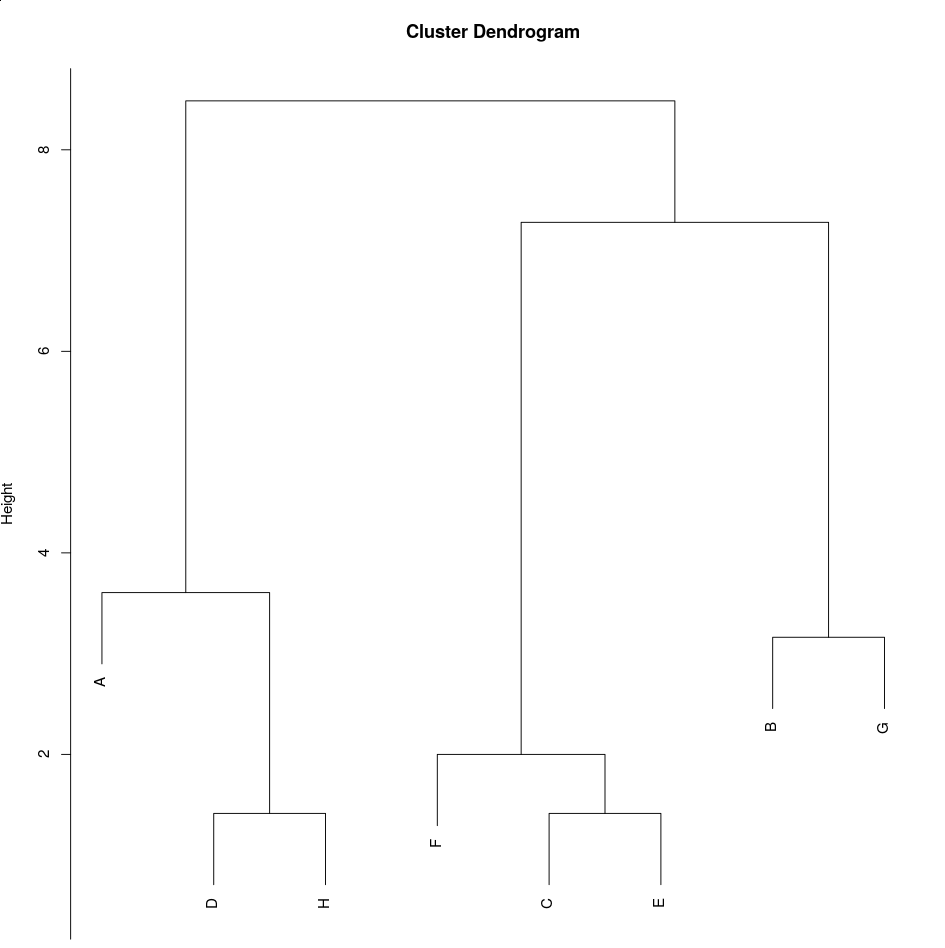
\includegraphics[width=\linewidth]{ClusterDendrogram.png}
\end{figure}

\end{document}







































